\documentclass[tikz,border=12pt]{standalone}
\usepackage[T1]{fontenc}
\usepackage{mathpazo}
\usepackage{amsmath,amssymb}
\usetikzlibrary{arrows.meta, positioning, calc}

\definecolor{stblue}{HTML}{7B97AD}
\definecolor{rwgold}{HTML}{B8995E}
\definecolor{sage}{HTML}{7A9A7E}
\definecolor{dkbrown}{HTML}{3D3530}
\definecolor{wmgray}{HTML}{7B7067}
\definecolor{cream}{HTML}{F9F6F0}
\definecolor{border}{HTML}{D4C9B8}
\definecolor{terracotta}{HTML}{C47A6A}

\begin{document}
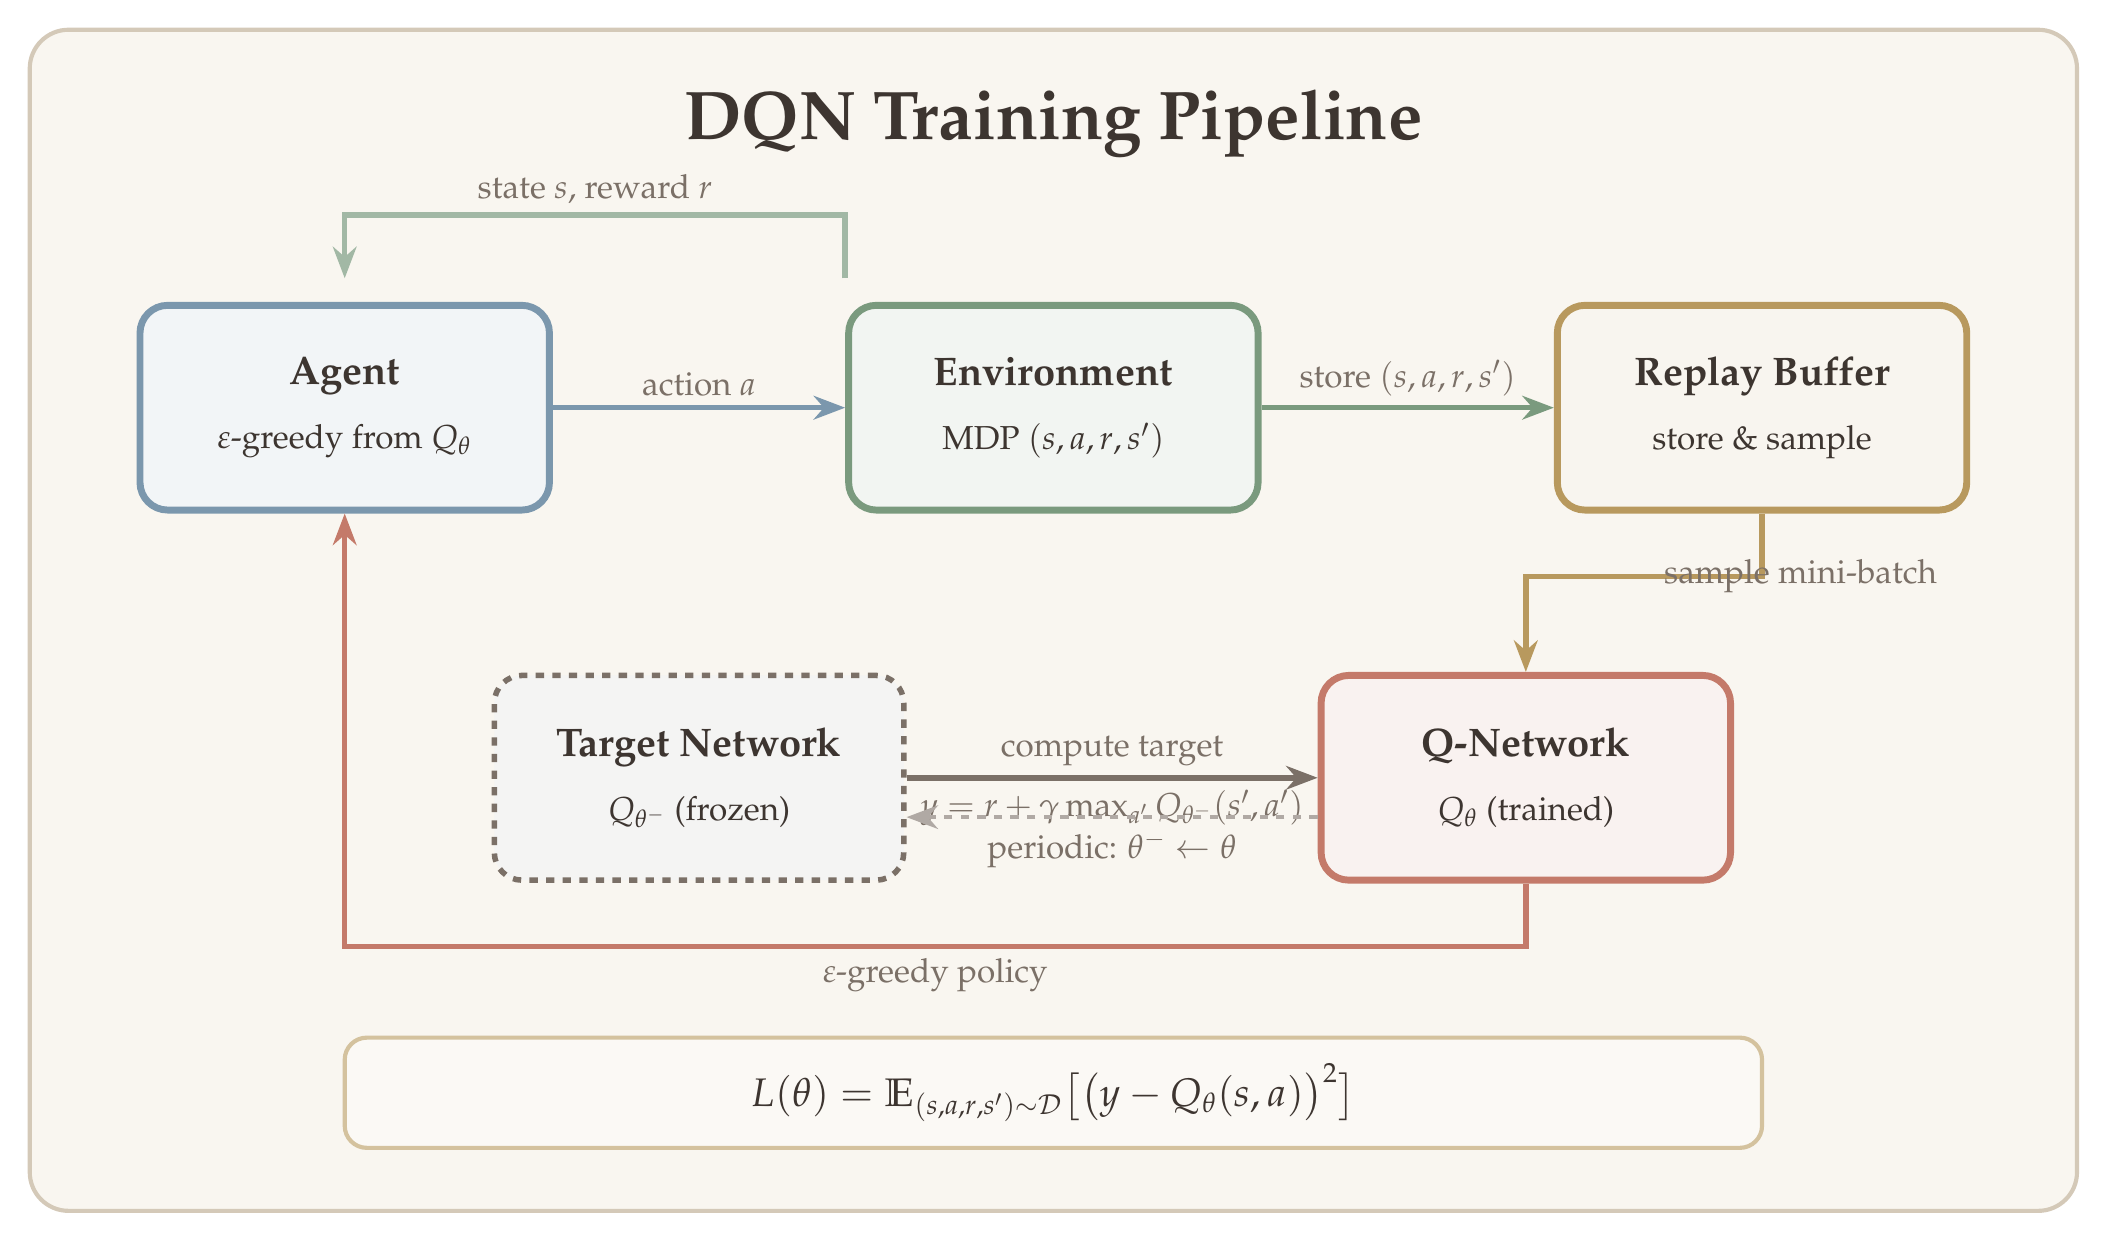
\begin{tikzpicture}[
  >={Stealth[length=4mm, width=3mm]},
  pbox/.style={
    draw=#1, line width=2.5pt, fill=#1!10, rounded corners=10pt,
    minimum width=52mm, minimum height=26mm, font=\Large, text=dkbrown,
    align=center, inner sep=8pt
  },
  arr/.style={->, line width=2pt, dkbrown},
  lbl/.style={font=\large, text=wmgray, align=center},
]

% Background
\fill[cream, rounded corners=14pt] (-2,-8) rectangle (24,7);
\draw[border, rounded corners=14pt, line width=1.5pt] (-2,-8) rectangle (24,7);

% Title
\node[font=\Huge\bfseries, text=dkbrown] at (11,5.8)
  {DQN Training Pipeline};

% =============================================
% Top row: Agent -- Environment -- Replay Buffer
% =============================================

\node[pbox=stblue] (agent) at (2,2.2)
  {\textbf{Agent}\\[5pt]
   {\large $\varepsilon$-greedy from $Q_\theta$}};

\node[pbox=sage] (env) at (11,2.2)
  {\textbf{Environment}\\[5pt]
   {\large MDP $(s,a,r,s')$}};

\node[pbox=rwgold] (buffer) at (20,2.2)
  {\textbf{Replay Buffer}\\[5pt]
   {\large store \& sample}};

% =============================================
% Bottom row: Target Network -- Q-Network
% =============================================

\node[draw=wmgray, line width=2pt, dashed, fill=wmgray!8,
      rounded corners=10pt, minimum width=52mm, minimum height=26mm,
      font=\Large, text=dkbrown, align=center, inner sep=8pt]
  (target) at (6.5,-2.5)
  {\textbf{Target Network}\\[5pt]
   {\large $Q_{\theta^-}$ (frozen)}};

\node[pbox=terracotta] (qnet) at (17,-2.5)
  {\textbf{Q-Network}\\[5pt]
   {\large $Q_\theta$ (trained)}};

% =============================================
% Arrows — clean layout
% =============================================

% Agent -> Environment: action
\draw[arr, stblue] (agent.east) -- (env.west)
  node[midway, above, lbl] {action $a$};

% Environment -> Buffer: store
\draw[arr, sage] (env.east) -- (buffer.west)
  node[midway, above, lbl] {store $(s,a,r,s')$};

% Environment -> Agent: state, reward (curved above)
\draw[arr, sage!70] ([yshift=3mm]env.north west) -- ++(0,0.8) -| ([yshift=3mm]agent.north)
  node[pos=0.25, above, lbl] {state $s$, reward $r$};

% Buffer -> Q-Network: sample
\draw[arr, rwgold] (buffer.south) -- ++(0,-0.8) -| (qnet.north)
  node[pos=0.25, right, lbl, xshift=3pt] {sample mini-batch};

% Q-Network -> Agent: policy (curved below)
\draw[arr, terracotta] (qnet.south) -- ++(0,-0.8) -| (agent.south)
  node[pos=0.25, below, lbl] {$\varepsilon$-greedy policy};

% Target -> Q-Network: compute target
\draw[arr, wmgray] (target.east) -- (qnet.west)
  node[midway, above, lbl] {compute target}
  node[midway, below, lbl] {$y = r + \gamma \max_{a'} Q_{\theta^-}(s',a')$};

% Q-Network -> Target: periodic copy (dashed, reverse)
\draw[->, line width=1.5pt, dashed, wmgray!60]
  ([yshift=-5mm]qnet.west) -- ([yshift=-5mm]target.east)
  node[midway, below, lbl, yshift=-1pt] {periodic: $\theta^- \leftarrow \theta$};

% =============================================
% Loss formula at bottom
% =============================================
\draw[rwgold!60, line width=1.5pt, rounded corners=8pt, fill=rwgold!6]
  (2,-7.2) rectangle (20,-5.8);

\node[font=\Large, text=dkbrown] at (11,-6.5)
  {$L(\theta) = \mathbb{E}_{(s,a,r,s') \sim \mathcal{D}}\bigl[
    \bigl(y - Q_\theta(s,a)\bigr)^2
  \bigr]$};

\end{tikzpicture}
\end{document}
